\documentclass[a4paper,12pt,twoside]{article}
\usepackage{IEM_2nd_Qtr}



\begin{document}

\thispagestyle{empty}

\begin{center}
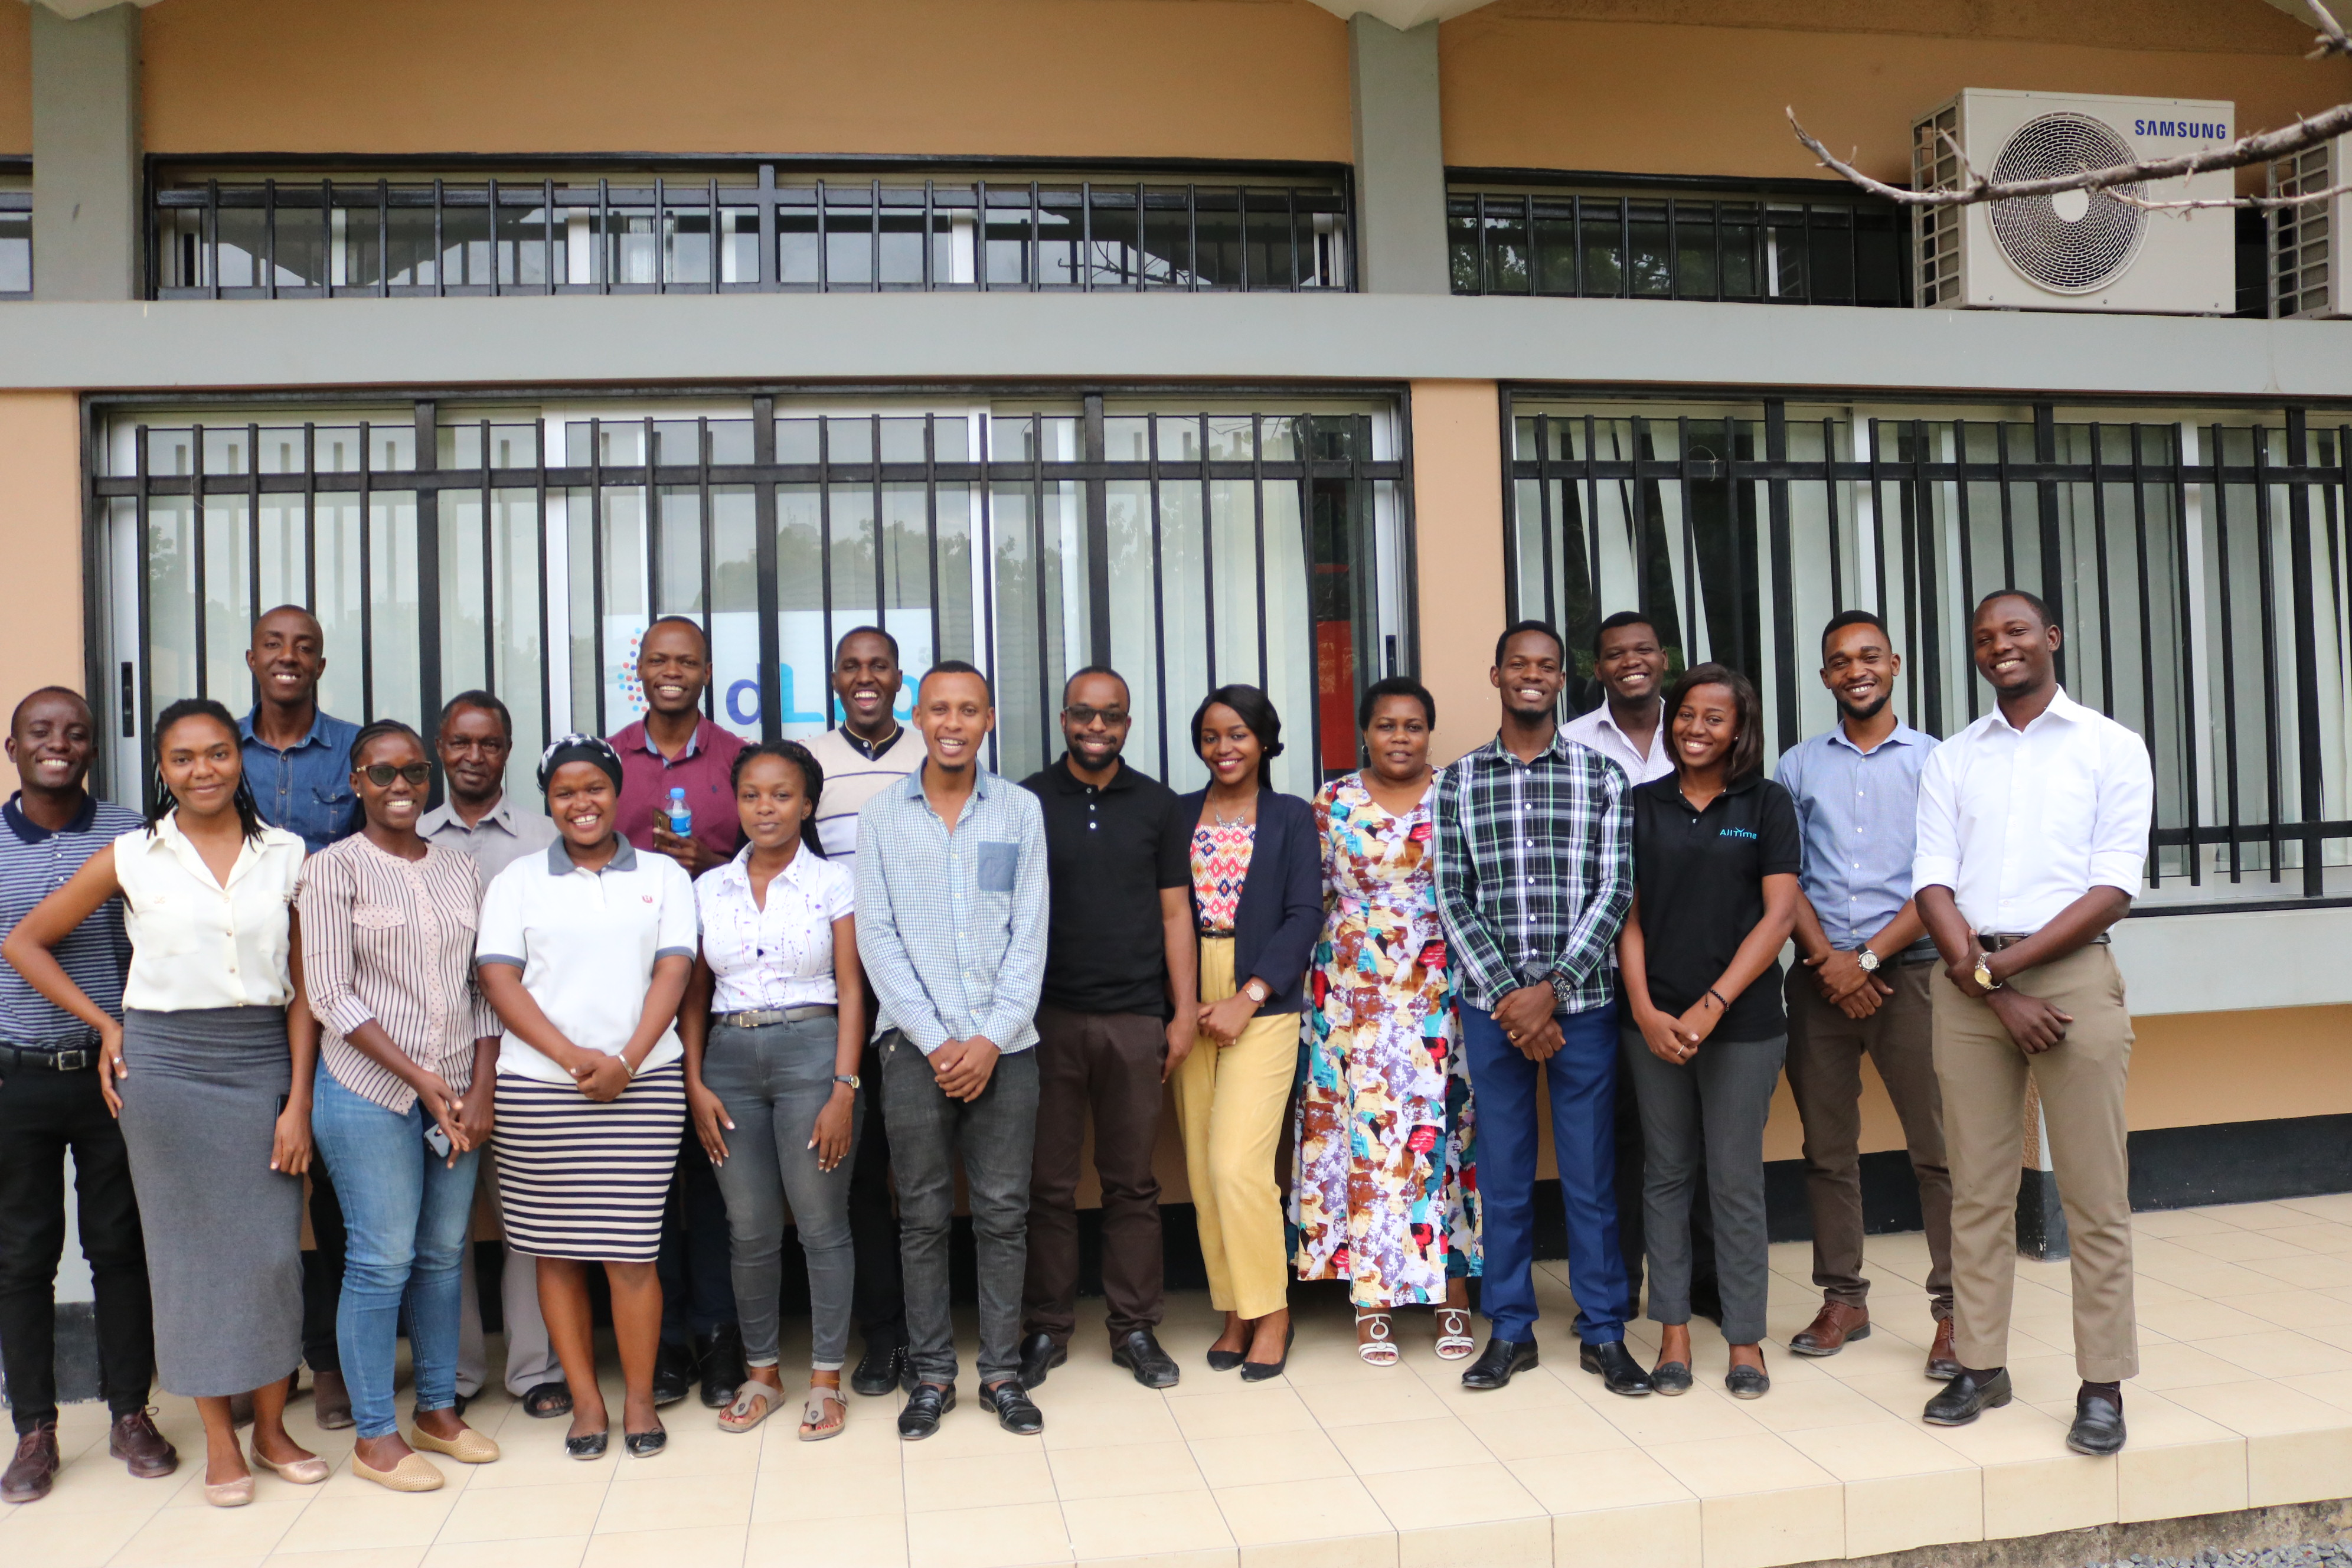
\includegraphics[width=\textwidth]{Group_shot.JPG}
\end{center}

\begin{center}
\bigskip
  \Huge 
\color{OMDTZblue} \textbf {Innovation Ecosystem Map}
\\
\textbf{Project Progress Report}
\\
\end{center}
\bigskip \bigskip \bigskip
\\
  \vbox{
  \centering
  Prepared for:
  \vcenteredhbox{
\includegraphics[width=2cm]{images/hdif_logo_new.png}}
  \
  by:
  \vcenteredhbox{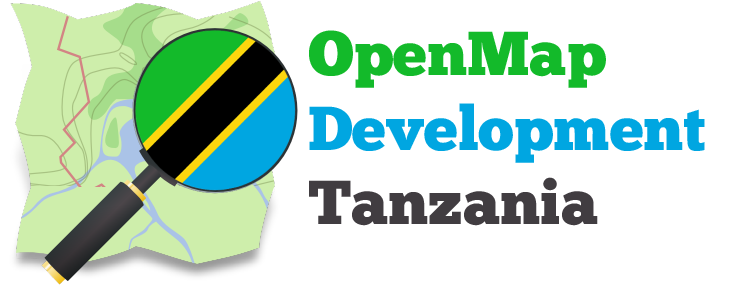
\includegraphics[width=4cm]{images/OpenMap_Development_TZ_Logo_Security_Card.png}}
  % \maketitle
}
\bigskip  \bigskip \bigskip
\begin{center}
  July 2019, Dar es Salaam, Tanzania  
  
 \bigskip \bigskip \bigskip \bigskip \bigskip \bigskip
\end{center}
 
\begin{flushleft}
	\footnotesize {\textbf{Authors:} Wombura Kimacha, Evarist Isdory, Johanes Peter, Hawa Adinani, Immaculate Mwanja and { } { } { } { } { } { } Innocent Maholi}
\end{flushleft} 
  

\newpage
\tableofcontents

\newpage
\section{Summary}
With the support from Human Development Innovation Fund (\href{http://www.hdif-tz.org/}{HDIF}\footnote{\url{http://www.hdif-tz.org/}}), OpenMap Development Tanzania(\href{http://omdtz.or.tz}{OMDTZ}\footnote{\url{http://omdtz.or.tz}}) has been tasked to review the technology and administer an innovation mapping platform as well as create community ownership of the platform by the innovation stakeholders in Tanzania. Administering the platform involves training innovation stakeholders to add relevant information to the map platform to facilitate collaborations and connect with each other to enable a conducive environment for innovators, for example, to interact with donors/funders or interact with fellow innovators to share experiences and work together in joint projects. Reviewing map technology involves making the map platform user-friendly and easy to interact with when using it.

This report describes the second quarter of the Innovation Ecosystem Map of Tanzania Project and deep dives into the activities conducted in the quarter. It provides an in-depth description of the activities done from April to July of 2019 including web development for the newly developed map, what we have learned so far from the engagement with stakeholders and the communication strategies used for sustainability of the Innovation Ecosystem Map of Tanzania.



\section{Milestones}
This section provides an overview of the project status with regards to conducted activities and their progress as well as describing the milestones:

\subsection{Web Development}
Since the beginning of the second quarter, OMDTZ team has worked on developing a new mapping platform to replace the previous \href{http://innovate.co.tz}{previous innovation-map}\footnote{\url{http://innovate.co.tz}} platform. Challenges with the previous map opened a way for decision to replace it, these include the following:

\begin{itemize}
    \item Complications to use filtering-feature that makes it hard for beginner-users of the map to use the map easily and efficiently.
    \item As the map functions as the “market” for fund-receivers, the map had no ability to provide analytic functionalities to show traffic to the mapped features eg. who has visited your hub, when etc.
\end{itemize}

\begin{figure}[h]
    \centering
    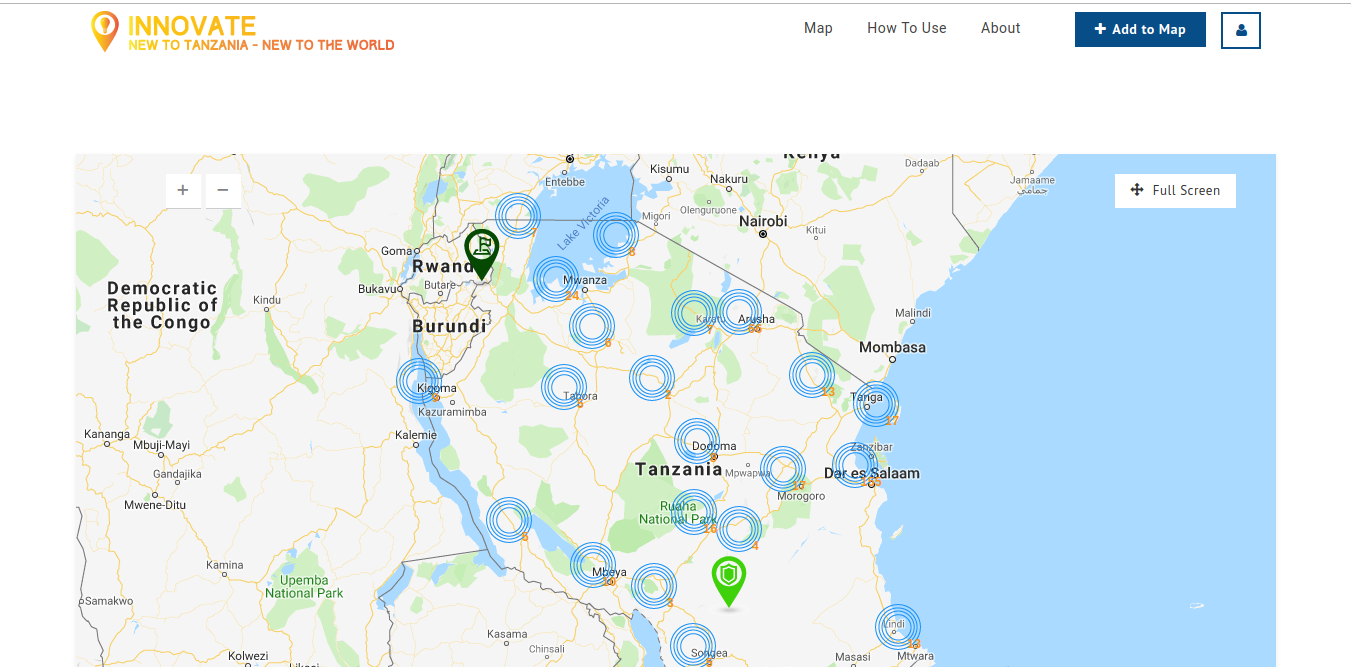
\includegraphics[width=0.9\textwidth]{old_inno_map.png}
    \caption{A layout of the old map platform on \href{innovate.co.tz}{innovate.co.tz}}
\end{figure}

With the above challenges in mind, development of the new mapping platform was carried out for a period of almost two months. The following activities were done during this period:


\begin{itemize}
	\item Research for main layout,
	\item Concept generation, prototyping
	\item Development, and lots of internal reviews to gain feedback and improve the platform
	\item External review with the HDIF which also helped improve the platform
\end{itemize}

On the fourth week of June, the new platform was completed awaiting reviews from the stakeholders during a mapathon. The \href{http://new.innovate.co.tz}{new map}\footnote{\url{http://new.innovate.co.tz}} is now accessible as seen in the images below:

\begin{figure}
	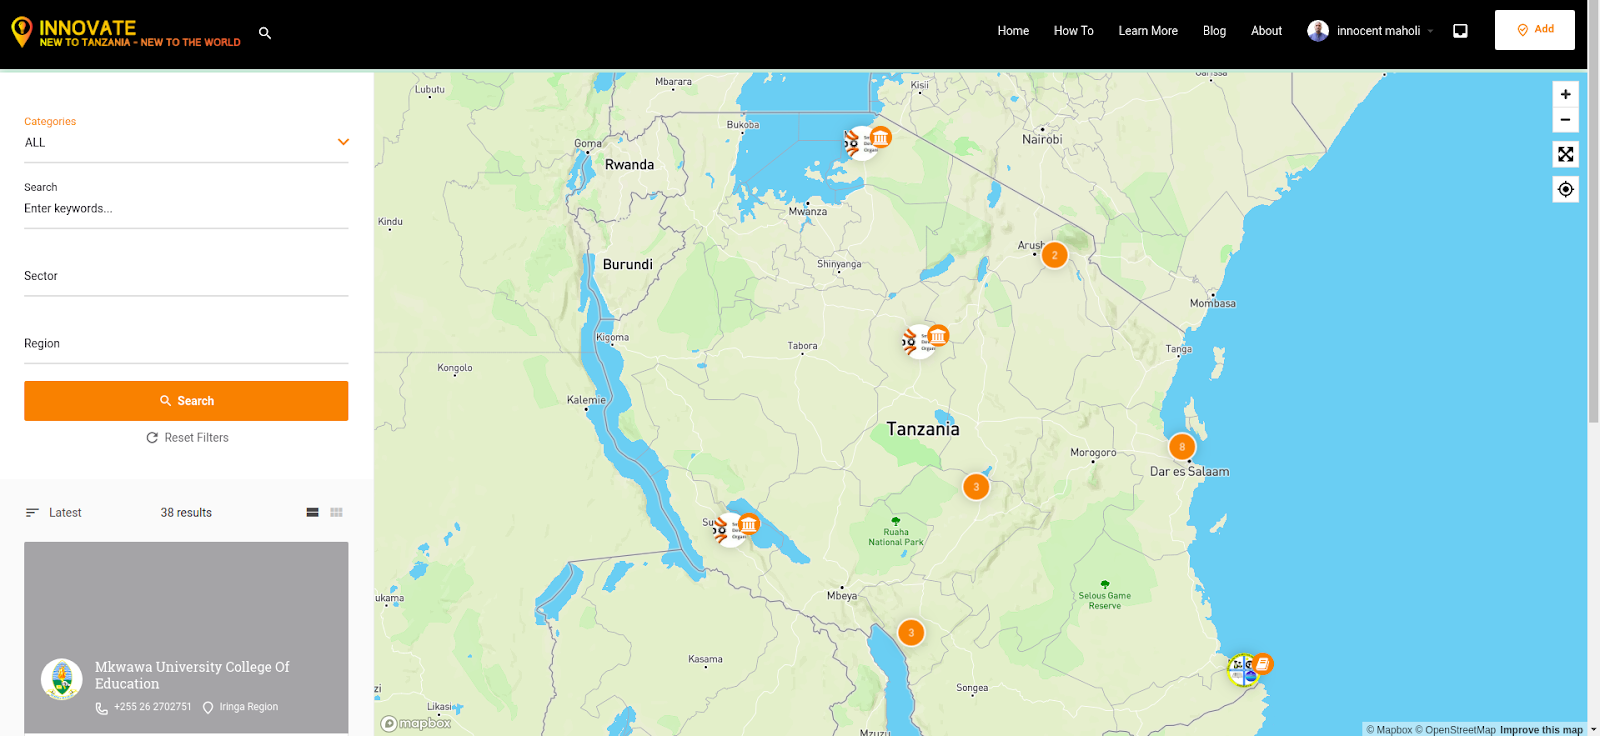
\includegraphics[width=0.9\textwidth]{images/new_new_inno_map.png}
	\caption{A layout of the new map platform on \href{http://new.innovate.co.tz}{new.innovate.co.tz }}
\bigskip \bigskip \bigskip \bigskip
	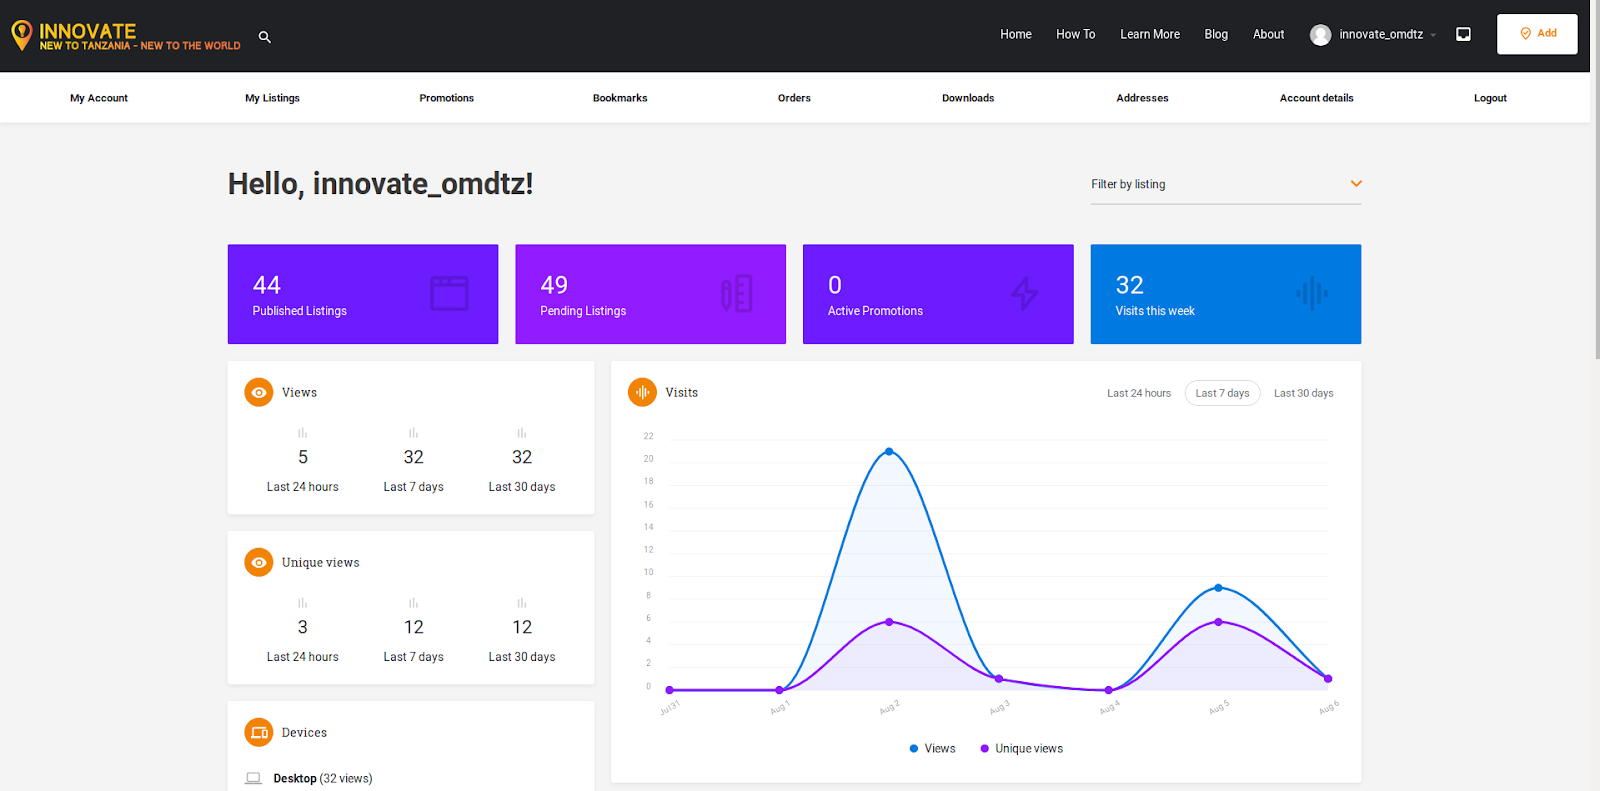
\includegraphics[width=0.9\textwidth]{images/dashboard.png}
	\caption{A layout of the new map platform user dashboard showing feature analytics }
\end{figure}

\newpage
\subsection{Training of Trainers}
OMDTZ in collaboration with HDIF, conducted a training for the trainers that took place on July 15th, 2019 at OMDTZ offices. The main objectives were to train mappers on how to conduct innovation mapathons and introduce them to travel guidelines that should be followed while in the field and to provide supervision and technical support to conduct the Innovation Ecosystem Map of Tanzania project in districts or regions during data collection.

Following the training that was provided in January 2019, the trainers were already familiar with the categories and contents of the Innovation Ecosystem of Tanzania. The training was collaborative as it provided room for interaction for every participant to give out comments and suggestions on the stakeholders, categories, sub-categories, and targeted groups on the map.  

It mainly focused on training the trainers who will be going out to the field all over Tanzania to hold mapathons and/or workshops with hub managers, innovators, teaching institutions, etc. in order to populate the map that is being developed.

\begin{figure}[H] % uncomment "[H]" to force the  image to the middle of the page  
	\centering
	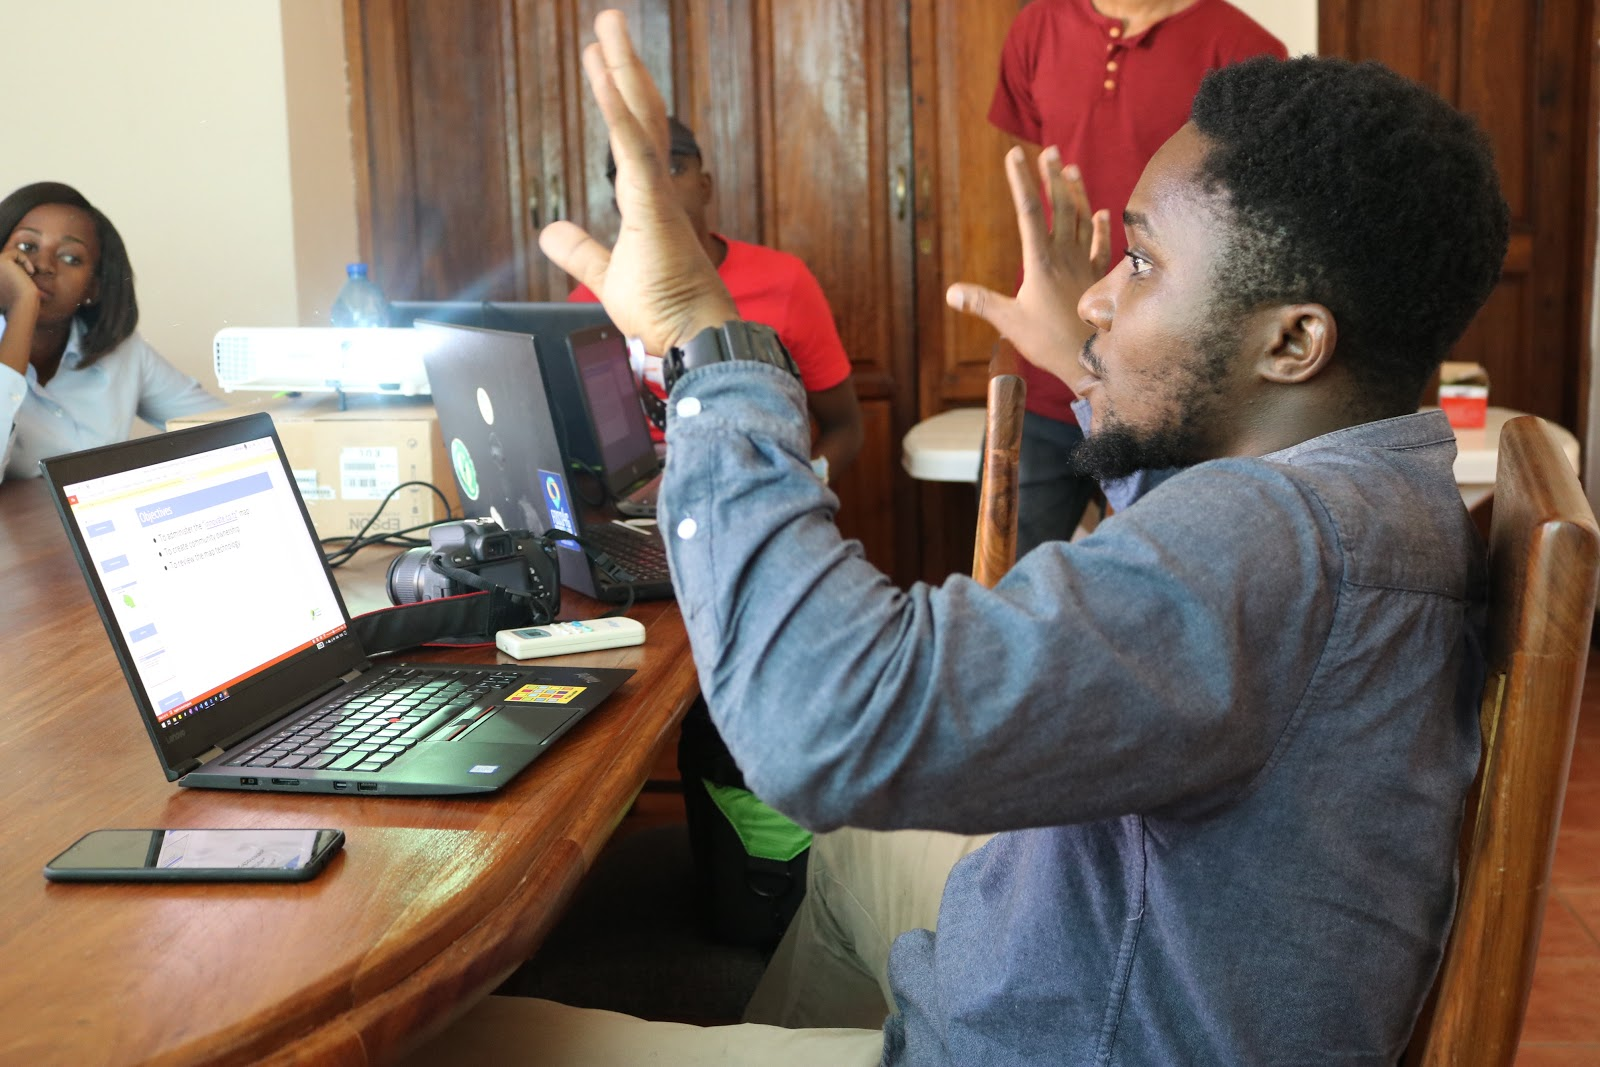
\includegraphics[width=0.9\textwidth]{images/Simon_training.JPG}
	\caption{Simon Mtabazi from the HDIF team commenting on the training of trainers held at OMDTZ office}
\end{figure}

The focus of the training was based on:

\begin{itemize}
	\item Introducing the trainers to travel guidelines that should be followed when in the field in districts and regions
	\item How to conduct mapathons with the involvement of innovation stakeholders in districts and regions of Tanzania
	\begin{itemize}
		\item How to register stakeholders and adding the listings of their categories
		\item Facilitate stakeholders in conducting their own mapathons and workshops that will be attended by the innovation stakeholders that could not be reached by the trainers
	\end{itemize}
	\item Introducing the trainers to the web map developed for the innovation ecosystem of Tanzania
	\item Preparing and planning for the mapathon
\end{itemize}

The training of trainers was succeeded by a mapathon that was conducted the next day on July 16, 2019.

\subsection{Mapathon}
This was a coordinated mapping event organized by OMDTZ with support from HDIF. The mapathon that was preceded by a training of trainers conducted the previous day, took place on July 16th, 2019 at OMDTZ’s partner \href{https://dlab.or.tz/}{Tanzania Data Lab}\footnote{\url{https://dlab.or.tz/}} Tanzania Data Lab (dLab) and was attended by 14 stakeholders from various innovation backgrounds, trainers and staff from OMDTZ and HDIF team members.

Participants of the mapathon were provided with Eventbrite tickets as notice prior to the mapathon in order to coordinate and prepare well. Before conducting the mapathon, OMDTZ contacted respective labs/hubs/universities and any other physical innovation space in Dar es Salaam that would participate in the mapathon.

The mapathon took approximately a maximum of 3 hours where the participants received full training on how to map themselves and used the time to actually map their organizations. What we learned is that most of the participants were familiar with the new map being developed by OMDTZ from the Hubs Manager’s workshop, exhibition, and presentations held during the Innovation Week of 25th - 30th of March, 2019.  

\begin{figure}%[H]
	\centering
	\caption{Mapathon conducted at Tanzania Data Lab}
	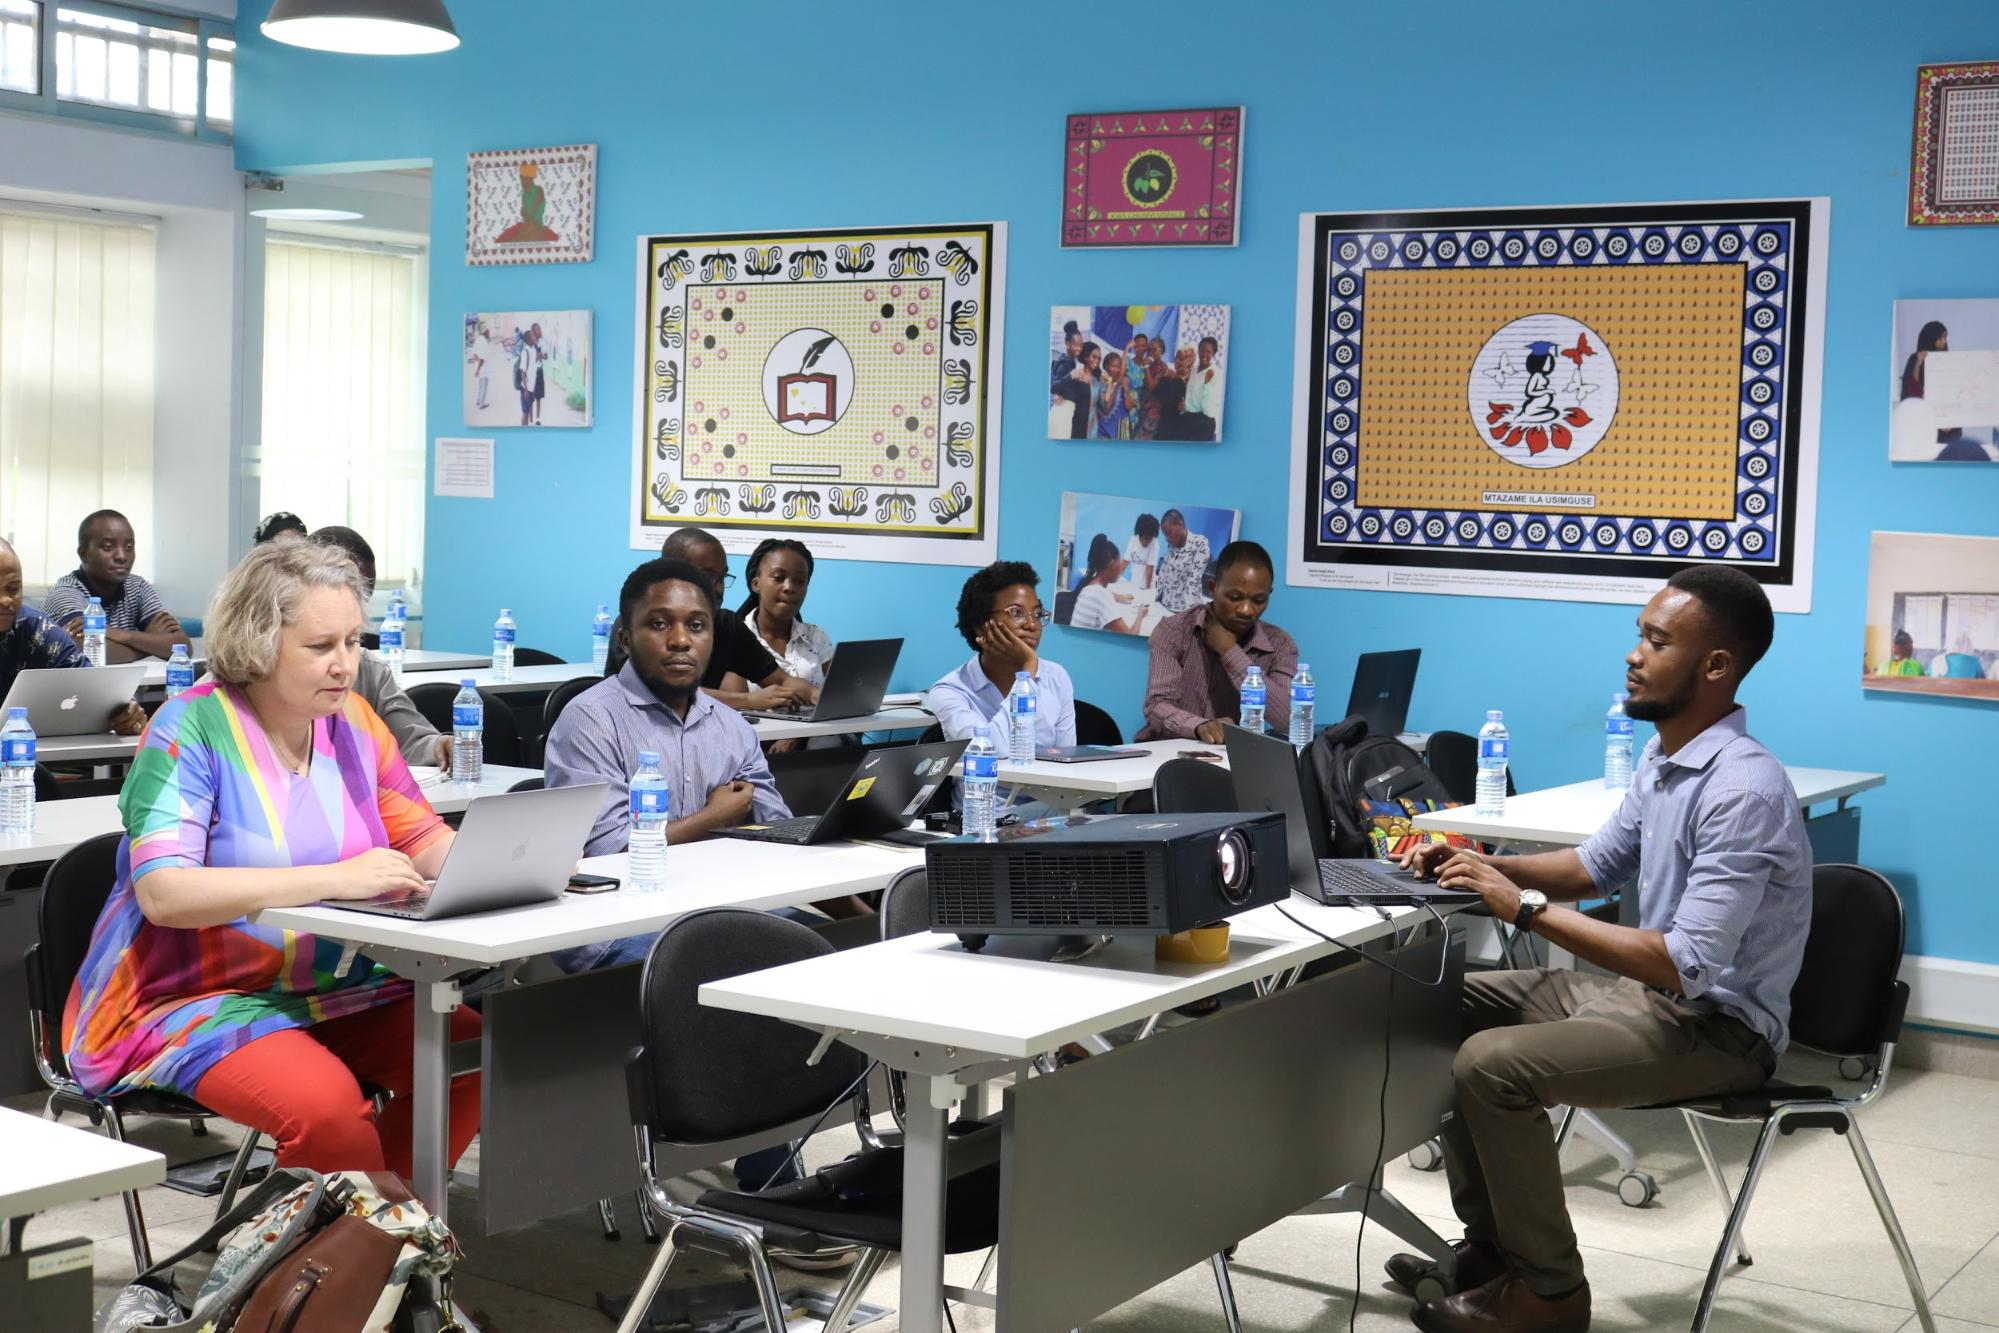
\includegraphics[width=0.8\textwidth]{mapathon.jpg}
\end{figure}

We got constructive feedback from the participants of the mapathon as all attendees agreed that all the categories that have been provided on the map are exhaustive enough. By the end of the training, the participants were asked to give feedback reflecting on the whole event. We intend to collaborate with more innovation stakeholders in the mapathons and workshops that will be held in the future to improve and make the innovation ecosystem map sustainable.

\section{Communications}
Communicating to the public about the map is the core activity that makes the Map popular and OMDTZ is committing to make that happen. Communicating to the public about the map is the core activity that makes the Map popular and OMDTZ is committing to make that happen. We have prepared a \href{https://docs.google.com/document/d/1E2_zR-vNxvte00CZwfj4i6A3WDjTw4HnVKfInVP6lpE/edit?usp=sharing}{draft communication strategy}\footnote{\url{https://docs.google.com/document/d/1E2_zR-vNxvte00CZwfj4i6A3WDjTw4HnVKfInVP6lpE/edit?usp=sharing}}---just for the map---that both teams from HDIF and OMDTZ are reviewing to finalize. The strategy will guide all communications about the project and the type of content to be shared.

The blog draft has been developed but not published yet as we are still waiting for reviews from HDIF's communications specialist. This will be published as soon as the communication strategy is finalized.

Also, during the innovation week, we had an opportunity to publicise the map to different stakeholders and featured on two media platforms---\href{https://youtu.be/o5rtxjeeLVI?t=55}{BBC News Swahili in Mitikasi Leo Show}\footnote{\url{https://youtu.be/o5rtxjeeLVI?t=55}} and ITV news (unfortunately, they could not upload the coverage to YouTube but was aired on the evening news)---where we introduced the map and explained why HDIF is interested on this platform and how it will be useful to the ecosystem of Tanzania's innovation.

\subsection{Social Media}
Handling multiple social media accounts is challenging especially when the accounts are not popular yet, therefore, in order to create good and reliable contents we decided to create only two social media accounts as a starting point.

We managed to create a \href{https://web.facebook.com/innovatetz}{Facebook page}\footnote{\url{https://web.facebook.com/innovatetz}} and \href{https://twitter.com/innovate_tz}{Twitter account}\footnote{\url{https://twitter.com/innovate_tz}} for the innovation ecosystem of Tanzania and have started posting about the map. Even though we have 63 followers on Twitter as of now, we are putting efforts to boost up our followers and engagement on social media. The image below shows the July engagement in Twitter, statistics and analytics 

\begin{figure}[h]
    \centering
    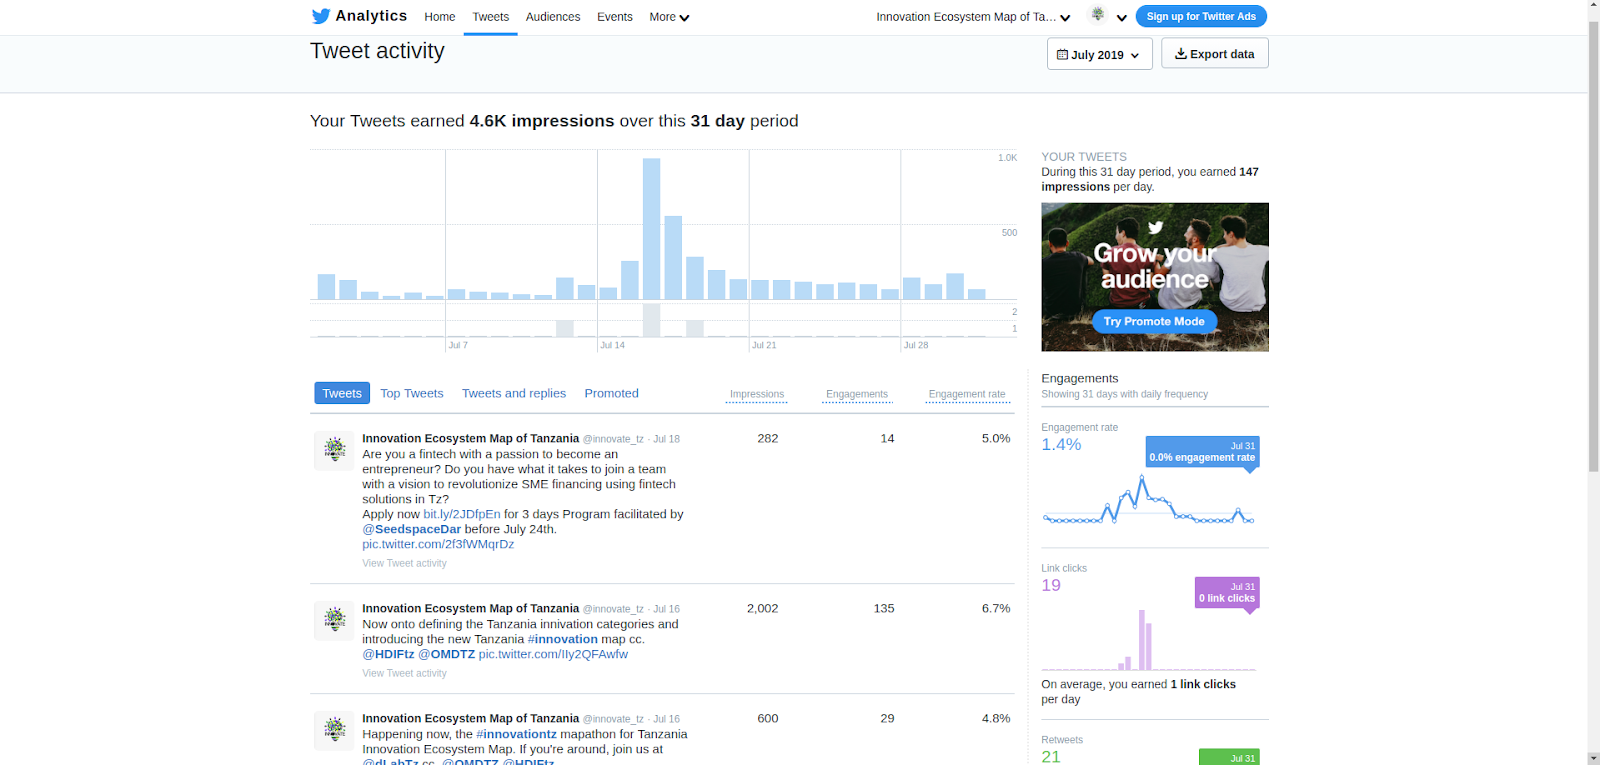
\includegraphics [width=1\textwidth]{tweet_activity.png}
\end{figure}

\newpage
\section{Learning and Challenges}
\textbf{\color{OMDTZblue}{Web Platform}}

The development of the platform took a much longer time to complete as a result of feedback from meetings with internal staff and our clients. Many components of the platform had to be changed overtime which led to the extension of completion time. Some of the reviews proposed the development of a different platform aside from the one that we made. Due to these frequent alterations of the platform, they swayed the direction of the platform development and other tasks had to stop waiting for its completion.

All suggestions provided in the reviews were for a good cause and improvement of the user experience and interface. As a result of frequent changes to the design of the platform, we did not get enough time to populate the map with stakeholders’ information as agreed. The map is going to be populated with data from both old platform and the new one. The task will be done by our mappers with 2 weeks of importation of data from the old platform and continuing with the collection of new data.

\textbf{\color{OMDTZblue}{Mapathon}}

For the second quarter, our work plan showed that 3 mapathons were to be conducted in Dar es Salaam, Arusha and Dodoma. One mapathon was conducted in Dar es salaam successfully on July 16th but we were not able to do the other two mapathons. This was a result of the feedback we received from the attendants of the event. We decided to cancel other mapathons and focus on fixing issues that we experienced with the new map platform such as crashing of the web platform. Currently, most of the comments that we received during the mapathon have worked.

Other challenges that were experienced during the mapathon include:
\begin{itemize}
    \item {\color{OMDTZblue}Internet connection:} During the beginning of the mapathon, the internet connection was poor but became stable as time went on. This caused a delay in some of the activities. In the next mapathons that will be conducted, we shall strive for a more stable connection and test it before we commence.
    
    \item {\color{OMDTZblue}Venue of the mapathon:} We delayed in booking the venue for the mapathon which posed as a challenge as we could not find a reliable (cost effective) venue at the very last minute with the limited time that we had left. In the future mapathons, a proper research on which venue should be used during mapathons will be conducted earlier and the booking will be done on time in order to avoid any future inconviniences.
    
    \item {\color{OMDTZblue}Attendance to the mapathon was lower than expected:} This is because invites to the attendees were sent later than our goal . Invites need to be sent at least 1 month before the event---with frequent reminder to the invitees---so they are aware of the upcoming events and can schedule their timetables accordingly.
\end{itemize}

\section{Financial Reporting}
Expenses breakdown:
\begin{figure}[h]
    \centering
    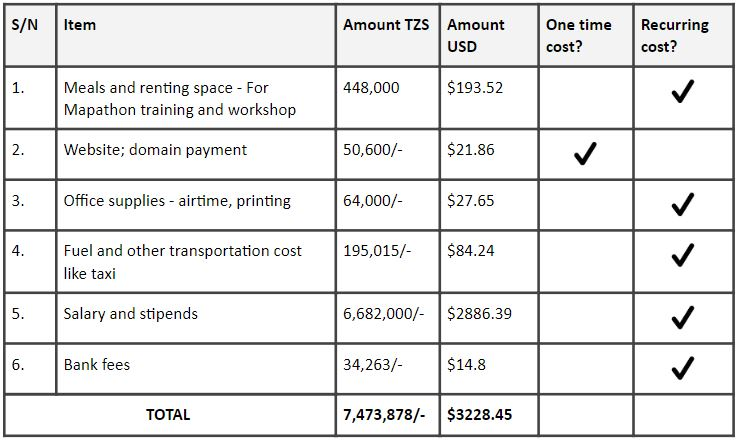
\includegraphics[width=0.9\textwidth]{images/finance.JPG}
\end{figure}


Second quarter opening and closing balance:
\begin{center}
	\begin{tabular}{|c|c|c|}
		\hline
		Item & TZS & USD \\
		\hline
		\rowcolor{Gray}
		Opening balance & 3,621,456/- & \$1,564.34 \\
	
		Amount advanced & 7,395,575/- & \$3,194.63 \\
		
		\rowcolor{Gray}
		Amount spent & 7,473,878/- & \$3,227.06 \\
		
		Balance in bank account + cash on hand & 3,543,153/- & \$1,530.51 \\
		\hline
	\end{tabular}
\end{center}

\end{document}
